\chapter{Closed orbits and tunes}\label{ch:orbits}

\section{Poincar\'e section and one-turn map}
In a static field with $N$-fold symmetry, the natural observable is the state of the particle each time it crosses a
fixed azimuth.
All benchmarks use the section $\theta = 0$ (the half-line $y = 0$, $x>0$) and the state
$X = (r, p_r, z, p_z)$ at fixed energy.
One turn of tracking defines the one-turn map $T: X\mapsto X'$.

\begin{figure}[h]
\centering
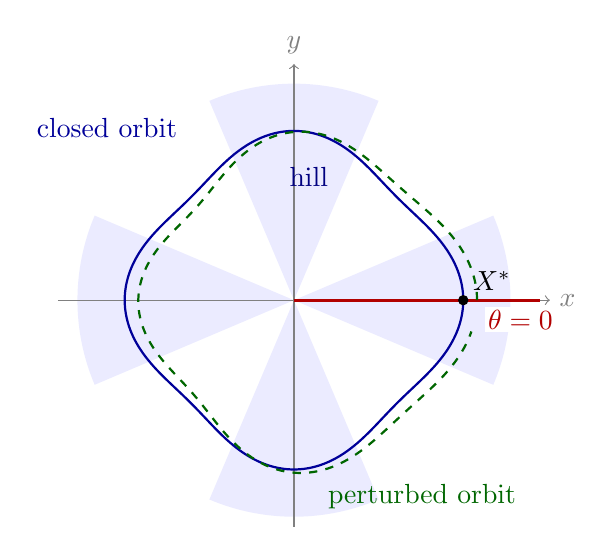
\begin{tikzpicture}[scale=1.25]
\foreach \k in {0,...,3} {
  \fill[blue!8,rotate=90*\k] (0,0) -- (-23:2.2) arc (-23:23:2.2) -- cycle;
}
\draw[->,gray] (-2.4,0) -- (2.6,0) node[right] {$x$};
\draw[->,gray] (0,-2.3) -- (0,2.4) node[above] {$y$};
\draw[very thick,red!70!black] (0,0) -- (2.5,0) node[pos=0.92,below=2pt,fill=white,inner sep=1pt] {$\theta=0$};
\draw[thick,blue!60!black,domain=0:360,samples=200,smooth,variable=\t]
  plot ({(1.6+0.12*cos(4*\t))*cos(\t)},{(1.6+0.12*cos(4*\t))*sin(\t)});
\draw[thick,green!40!black,dashed,domain=0:350,samples=200,smooth,variable=\t]
  plot ({(1.6+0.12*cos(4*\t)+0.14*cos(1.05*\t))*cos(\t)},{(1.6+0.12*cos(4*\t)+0.14*cos(1.05*\t))*sin(\t)});
\fill (1.72,0) circle (1.5pt) node[above right] {$X^*$};
\node[blue!60!black] at (-1.9,1.75) {closed orbit};
\node[green!40!black] at (1.3,-2.0) {perturbed orbit};
\node[blue!50!black] at (0.15,1.25) {hill};
\end{tikzpicture}
\caption{Section $\theta = 0$ in a 4-sector field.
The closed orbit is scalloped with the field period, farthest out in the hills, and crosses the section at the fixed
point $X^*$.
A perturbed orbit oscillates around it; the number of oscillations per turn is the tune.}
\label{fig:section}
\end{figure}

\paragraph{Crossing the section.}
The integrator does not land on $\theta = 0$.
The benchmark harness interpolates the crossing in time between steps: four-point Lagrange interpolation of the
full-step positions and momenta.
LIONS keeps momenta at half steps, so the harness forms full-step momenta by a half Boris kick of $\vect p^{\,n-1/2}$.
That is the exact inverse of the start-up, so the recorded map is conjugate to the Boris map.
The interpolation is not symplectic, and its error is $O(\Delta t^4)$.
At 1440 steps per turn it is below the finite-difference noise of the Jacobian.

\section{Closed orbit}
The closed orbit is the fixed point $T(X^*) = X^*$.
Finding it by Newton iteration on the one-turn map, and reading the focusing from the one-turn matrix, is the classic
method of cyclotron orbit codes \cite{gordon1984}.
Newton's method on $G(X) = T(X) - X$ iterates
\begin{equation}
X_{k+1} = X_k - (M_k - I)^{-1}\,\big(T(X_k)-X_k\big),\qquad M_k = \frac{\partial T}{\partial X}(X_k),
\end{equation}
with $M$ from central differences:
\begin{equation}
M_{:,j} \approx \frac{T(X+h\,e_j) - T(X-h\,e_j)}{2h}.
\end{equation}
The Newton iteration uses $h = \SI{1e-7}{m}$ on the radial block.
The Jacobian used for tunes and $\det M$ uses $h = \SI{1e-6}{m}$ in positions and $h\,p/\rho$ in momenta (the same step
as an angle $h/\rho$).
The truncation error is $O(h^2)$ and the rounding error is $O(\varepsilon_T/h)$, with $\varepsilon_T$ the noise of the
one-turn map.
A discrete one-turn map that is only piecewise smooth breaks this picture: if a probe pair $X\pm he_j$ straddles a change of
slope, the difference quotient mixes two slopes, at any $h$.

\section{Tunes from the one-turn matrix}
In uncoupled planes $M$ is block-diagonal, with $2\times2$ blocks $M_r$, $M_z$.
For a symplectic block with $|\operatorname{tr}M_u|<2$ (stable motion), $\det M_u = 1$ and the block can be written in
Twiss form (here $\alpha$, $\beta$, $\gamma$ are the Twiss parameters, not the Lorentz factors)
\begin{equation}
M_u = I\cos\mu + \begin{pmatrix}\alpha & \beta\\ -\gamma & -\alpha\end{pmatrix}\sin\mu,\qquad
\cos\mu = \tfrac12\operatorname{tr}M_u,\qquad \mu = 2\pi Q_u
\end{equation}
\cite{courant1958}.
The trace only fixes $\cos 2\pi Q$: it gives the fractional tune, folded into $[0, 0.5]$.
Its sensitivity is
\begin{equation}
\delta Q = -\frac{\delta(\operatorname{tr}M)}{4\pi\sin 2\pi Q},
\end{equation}
which diverges near $Q\in\{0, 0.5\}$.
This is why the PSI energies where $\Qr$ crosses $1.5$ are reported separately.

When $\det M_u\ne1$, the trace formula still returns a number, but it no longer is the tune of an area-preserving
oscillation; the consistent definition is then $\cos\mu = \operatorname{tr}M_u/(2\sqrt{\det M_u})$.
The benchmark harness uses $\operatorname{tr}M_u/2$.
A $\det M_u - 1$ of \GPsiLionsDetMed{} (median), as found for LIONS on the PSI map, means the formula is used outside its validity.

\section{Conditioning of the closed orbit}\label{sec:conditioning}
For an area-preserving block,
\begin{equation}
\det(M_u - I) = 2 - \operatorname{tr}M_u = 4\sin^2(\pi Q_u).
\end{equation}
A map error $\delta$ moves the fixed point by $(I-M_u)^{-1}\delta$.
In normalised coordinates $M_u$ is a rotation by $2\pi Q_u$, and $\|(I-M_u)^{-1}\| = 1/(2\sin\pi Q_u) = 1/\sqrt{\det(M_u-I)}$:
the classic $\beta/(2\sin\pi Q)$ closed-orbit sensitivity.
The sensitivity grows as $1/\sqrt{\det(M_u-I)}$, not as $1/\det(M_u-I)$.
In case B, with a fractional $\Qr$ of \BLionsQr, $\det(M_r-I) = \BCondDet$ and the amplification is about \BSens{} in
normalised units.
This near-integer amplifier (hypothesis H4) was a candidate for the case B scatter (\cref{sec:caseB}).

\section{Tunes from tracking}
A second instrument: track a particle offset by \SI{1e-4}{m} from the closed orbit for 256 turns, record the
turn-by-turn signal, apply a Hann window, and take the frequency that maximises the windowed discrete Fourier transform.
The maximum is refined by golden-section search.
Windowing and interpolating the spectrum peak gives a frequency resolution much finer than $1/N_{\rm turns}$
\cite{bartolini1996}.
On case B0 the two instruments agree within \BzeroFFTAgree.
